%%%%%%%%%%%%%%%%%%%%%%%%%%%%%%%%%%%%%%%%%%%%%%%%%%%%%%%%%%%%%%%%%%%%%%%%%%%%%%%%
\documentclass[twocolumn]{revtex4}

%%%%%%%%%%%%%%%%%%%%%%%%%%%%%%%%%%%%%%%%%%%%%%%%%%%%%%%%%%%%%%%%%%%%%%%%%%%%%%%%
% Note that comments begin with a "%" and are not turned into text in the .pdf
% document.
%%%%%%%%%%%%%%%%%%%%%%%%%%%%%%%%%%%%%%%%%%%%%%%%%%%%%%%%%%%%%%%%%%%%%%%%%%%%%%%%

%%%%%%%%%%%%%%%%%%%%%%%%%%%%%%%%%%%%%%%%%%%%%%%%%%%%%%%%%%%%%%%%%%%%%%%%%%%%%%%%
% Include some extra packages.
%%%%%%%%%%%%%%%%%%%%%%%%%%%%%%%%%%%%%%%%%%%%%%%%%%%%%%%%%%%%%%%%%%%%%%%%%%%%%%%%
\usepackage[]{graphicx}
%%%%%%%%%%%%%%%%%%%%%%%%%%%%%%%%%%%%%%%%%%%%%%%%%%%%%%%%%%%%%%%%%%%%%%%%%%%%%%%%

%%%%%%%%%%%%%%%%%%%%%%%%%%%%%%%%%%%%%%%%%%%%%%%%%%%%%%%%%%%%%%%%%%%%%%%%%%%%%%%%
\begin{document}

%%%%%%%%%%%%%%%%%%%%%%%%%%%%%%%%%%%%%%%%%%%%%%%%%%%%%%%%%%%%%%%%%%%%%%%%%%%%%%%%
\title{
Can You Escape a Velociraptor?
}

\author{Fred Genier}
\affiliation{Siena College, Loudonville, NY}

\date{\today}

\begin{abstract}
    For the final project of CSIS 200, we have been tasked with using Python to figure out if a human, with a 30 meter head start, could escape a velociraptor. This was determined in four steps: Graphing the position vs. time of both the human and velociraptor, calculating the time to intercept, calculating the time until the velociraptor could strike, and finally calculating the probability of escape. It was determined that, under the given circumstances, a human could escape the velociraptor roughly 60\% of the time.
\end{abstract}

\maketitle
%%%%%%%%%%%%%%%%%%%%%%%%%%%%%%%%%%%%%%%%%%%%%%%%%%%%%%%%%%%%%%%%%%%%%%%%%%%%%%%%

%%%%%%%%%%%%%%%%%%%%%%%%%%%%%%%%%%%%%%%%%%%%%%%%%%%%%%%%%%%%%%%%%%%%%%%%%%%%%%%%
\section{Position vs. Time}
%%%%%%%%%%%%%%%%%%%%%%%%%%%%%%%%%%%%%%%%%%%%%%%%%%%%%%%%%%%%%%%%%%%%%%%%%%%%%%%%

	The first task was to create a position vs. time graph for both the raptor and the human. This would help to roughly approximate when the velociraptor would catch up to the human. The equation used to plot followed the basic $y=mx+b$ format. The $y$-value would be the distance traveled by the subject, $x$ would be time, $m$ would be velocity, and $b$ would be starting position, if any.
	
	The velociraptor's given speed was 18 $m/s$ and had a starting position of zero, so the equation for its motion would be:
	$$y=18x+0$$
	The human's given speed was 3 $m/s$ and had a head start of 30 meters, so the equation for its motion would be:
	$$y=3x+30$$
	To graph these using python, two variables were set equal to the previously mentioned equations. The $x$-value was set equal to a numpy array containing a range of 0-5. With this, when run, the equation would generate every $y$-coordinate from $t=0$ to $t=5$. Both variables were plotted against the $x$-array, and this was the resulting plot:
	\begin{figure}
		\centering
		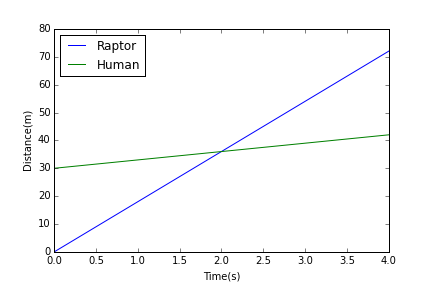
\includegraphics[width=.9\linewidth]{./graph1}
		\label{fig:graph1}
	\end{figure}
%%%%%%%%%%%%%%%%%%%%%%%%%%%%%%%%%%%%%%%%%%%%%%%%%%%%%%%%%%%%%%%%%%%%%%%%%%%%%%%%
\section{When does the raptor catch up to you?}
%%%%%%%%%%%%%%%%%%%%%%%%%%%%%%%%%%%%%%%%%%%%%%%%%%%%%%%%%%%%%%%%%%%%%%%%%%%%%%%%

	The second task was to determine exactly when the velociraptor would catch up to the human. Unlike the first tast, an algebraic method was not used here. Essentially, the task was to figure out when the distance travelled by the human and the distance traveled by the velociraptor was equal.
	
	In order to determine this, a relatively simple python function was used. The function would take in each $y$-value and a range, and would output the time it took for the raptor to catch up, and the distance the human had travelled when it did.
	
	The function would compare the $y$-values of each subject at each time interval, and when they were equal it would output the time interval at which both were equal and the distance the human subject traveled.
	
	When run, the function output that it would take 2 seconds for the raptor to catch up, after the human had run 6 meters.
%%%%%%%%%%%%%%%%%%%%%%%%%%%%%%%%%%%%%%%%%%%%%%%%%%%%%%%%%%%%%%%%%%%%%%%%%%%%%%%%
\section{When is it close enough to strike?}
%%%%%%%%%%%%%%%%%%%%%%%%%%%%%%%%%%%%%%%%%%%%%%%%%%%%%%%%%%%%%%%%%%%%%%%%%%%%%%%%

	The third task was to determine how far the human subject had run and how much time had passed when the velociraptor was 1 meter behind it. The algebraic solution to this would be as follows:
	
	$$t_{strike}=\frac{d_{human}-1}{v_{raptor}}$$
	$$d=t_{strike}*v_{human}$$
	
	In order to determine this using Python, a simple function was made that would essentially do this algebra. The function would take in the $y$-value at which the human and velociraptor's position was equal and the velocity of the raptor. It would then subtract 1 from the position and divide by the velociraptor's speed. To determine the distance travelled by the human, this time value would simply be multiplied by 3 (the human's velocity).
	
	All said and done, the function reported that the raptor would be able to strike after 1.94 seconds, at which point the human had travelled 5.83 meters.

%%%%%%%%%%%%%%%%%%%%%%%%%%%%%%%%%%%%%%%%%%%%%%%%%%%%%%%%%%%%%%%%%%%%%%%%%%%%%%%%
\section{Will it bite you?}
%%%%%%%%%%%%%%%%%%%%%%%%%%%%%%%%%%%%%%%%%%%%%%%%%%%%%%%%%%%%%%%%%%%%%%%%%%%%%%%%

	Perhaps the most difficult task, the final one was to determine whether or not the raptor would bite you when it was finally in range to strike. According to the question, it would attempt to bite three times, each with a varying probability of success. The first bite would have a 20\% chance to succeed, the second would have a 15\% chance, and the third would have a 7\% chance. If all three bites failed, the human escaped.
	
	In order to solve this using Python, an initial function was created to simulate these three bites. Each bite was declared as a variable, which was equal to a random integer between 1 and 100. For the first bite, if the integer was less than or equal to 20, the bite succeeded and vice versa. This was the same procedure used for the second and third bites, only with the second and third the critical number was 15 and 7, respectively. If any of the bites succeeded, the function would return an "f" and if none of them did, it would return an "s".
	
	With the function to simulate the escape, it needed to be run many times to determine the probability of escape. Two variables were declared, "successes" and "failures", to count how many successes and failures the function returned. Using a for loop, the function was then run 10,000 times and a rough percentage was calculated by rounding to the nearest whole number. Though it varies, the percentage tends to stay around 61\%.
	
	

%%%%%%%%%%%%%%%%%%%%%%%%%%%%%%%%%%%%%%%%%%%%%%%%%%%%%%%%%%%%%%%%%%%%%%%%%%%%%%%%
\end{document}
%%%%%%%%%%%%%%%%%%%%%%%%%%%%%%%%%%%%%%%%%%%%%%%%%%%%%%%%%%%%%%%%%%%%%%%%%%%%%%%%
